\chapter{Task: implementing a neural network Q-table} \label{ch:neural_networks}
For this project a neural network must be used to approximate the value function for the agent. This is due to the large size of the dominion state space as discussed in chapter \ref{sec:engine_implementation}. This chapter will discuss all the details of the implemented neural network, which is identical for all agents.

\section{Neural network structure}
\begin{figure}[H]
    \centering
    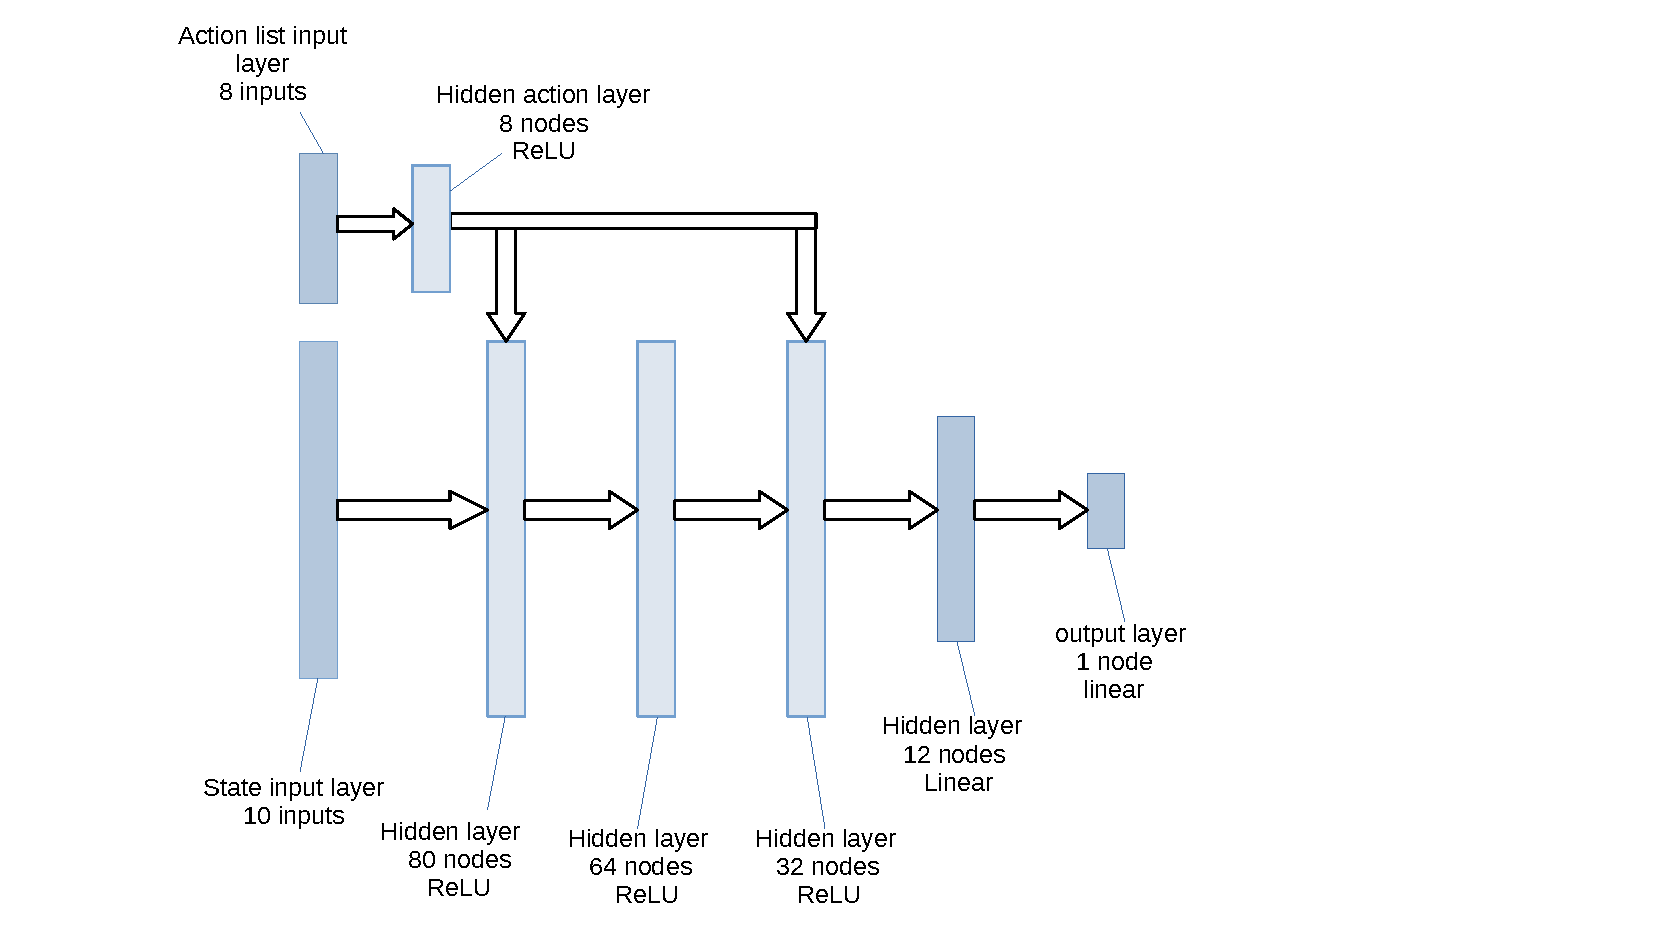
\includegraphics[width=0.8\textwidth]{img/NN_model.pdf}
    \caption{The neural network structure used for the agents.}
    \label{fig:neural_network}
\end{figure}
As shown in the neural network then the action values are fed into the neural network, as a residual connection. This is due to the fact, that it was observed that the actions has little value for the final result of the value function. As the actions are also passed in later in the neural network, the symbolic representation of the actions are represented stronger in the final output. Furthermore, it should also be noted, that a significant finding, was that the ReLU activation function was better than any other activation function tested. This is most likely due, to the fact, that the ReLU has an infinite range of positive values, which is beneficial for the value function. Though it should also be noticed, that the two last layers use linear layers, as the output of the value function should support being any number between -$\infty$ and $\infty$.\\\\
Using this neural network structure then it is time for the agents to train on the Dominion game. This will be discussed in the next chapter.
For the rest of this chapter, then the design choices for the neural network will be explained. 

\subsection{Residual action layer connection}
It was shown through experience, that the influence of the action input was insignificant for all states that the agent was trained in. Meaning that given a state, then all actions would suffice to the same Q-table value. This feature prohibited learning the concept of good actions, and had to be dealt with. To enlarge the importance of the action input, then the final neural network design made use of residual connections in which the action input was also added into the neural network later in the hidden layers. The intuitive idea, was that the action input would influence the final output greater, if the action input was also given at a later stage of the neural network, to make sure it does not vanish. This approach solved the problem of identical Q-table values for all actions. 

\subsection{Binarization of the action layer input}
At this point of the neural network design, it was decided to use one integer value as the action input, instead of the 8 values used now. The agent was now capable of learning the value difference between actions. But another problem was observed. It was observed, that the neural network would learn a dependency between action index and the value of the action. This dependency would incorrectly influence the value function. An example was the action to buy a "curse" card, which in practically all cases would be a bad choice. This action is numerically adjacent to buying the "province" card, which in practically all cases would be a good choice to buy if possible. Since the "province" card rarely was bought due to its expensive price, then the neural network would learn that the "province" card probably was a bad choice, since it was numerically close to the "curse" card.\\

To mitigate the spatial relation between actions, then the action input was binarized. action 1 would then be represented as [1, 0, 0, 0, 0, 0, 0, 0], action 3 as [1, 1, 0, 0, 0, 0, 0, 0] and so on. Furthermore, a hidden layer, exclusively for the action input was added.
This approach removed the spatial relation between actions giving each action an appropriate value. 

\subsection{Optimistic initialization}
To improve the explorative nature of the agent, then the weights of the neural network was initialized optimistically. Intuitively, then the agent would try new states with greater probability before realizing that the state was bad. Specifically the neural network weights was optimistically initialized by setting them based on a normal distribution with variance 0.01 and mean 0.05 